%Technick� univerzita v Ko�iciach, Fakulta elektrotechniky a informatiky
%Katedra po��ta�ov a informatiky
%\renewcommand{\contentsname}{Whatever}

%\documentclass[12pt]{article}
\documentclass[parskip=full]{scrartcl}
\usepackage[slovak]{babel}
\usepackage{slovak}
\usepackage[cp1250]{inputenc}
\usepackage[T1]{fontenc}
\usepackage[pdftex]{graphicx}
\usepackage{url}
\usepackage{verbatim} 
\usepackage{lipsum}% just to generate text for the example

\usepackage{fancyhdr}
\usepackage{lastpage}

%\usepackage{hyperref}
%\hypersetup{pdftex,colorlinks=true,allcolors=blue}
%\usepackage{hypcap}
%\begin{comment}
\usepackage[]{hyperref}
\hypersetup{
    pdftitle={Your title here},
    pdfauthor={Your name here},
    pdfsubject={Your subject here},
    pdfkeywords={keyword1, keyword2},
    bookmarksnumbered=true,     
    bookmarksopen=true,         
    bookmarksopenlevel=1,       
    colorlinks=true,            
    pdfstartview=Fit,           
    pdfpagemode=UseOutlines,    % this is the option you were lookin for
  %  pdfpagelayout=TwoPageRight
}
%\end{comment}
\pagestyle{fancy}
\lhead{\footnotesize \parbox{11cm}{Riddle} }
\lfoot{\footnotesize \parbox{11cm}{\textit{Technick� univerzita v Ko�iciach, Fakulta elektrotechniky a informatiky , 2012}}}
\cfoot{}
\rhead{\footnotesize }
\rfoot{\footnotesize Page \thepage\ of \pageref{LastPage}}
\renewcommand{\headheight}{24pt}
\renewcommand{\footrulewidth}{0.4pt}
\setlength{\parindent}{1cm}


\title{Riddle\\ Webov� technol�gie}
\author{
				\\\\\\\\\\\\\\\\\\autori:\\
         Bc. �ubom�r Rem�k \\
          % \and
        Bc. Patrik Ragan\\
         %\and
         Bc. Vojtech Rin�k\\
   \\
   \\
   \\
   \\
   \\
   \\
}
\date{\today}

\begin{document}
\maketitle

\newpage
\tableofcontents
\newpage

%uvod
\section{�vod}


~~~~~Webov� aplik�cia Riddle m� sl��i� ako pom�cka pre u�ite�ov po�as predn�ok. Predn�aj�ci
u�ite� si bude m�c� vytvori� ot�zku a zverejni� ju a n�sledne na �u bud� m�c� �tudenti odpoveda�, s mo�nos�ou
anonymnej odpovede. Potom si m��e u�ite� zobrazi� vyhodnotenia v textovej alebo grafickej
podobe.


\begin{figure}[h!]
\centering

\includegraphics[scale=0.50]{pics/riddleLogoH.png}
\end{figure}
%prieskum trhu
\section{Prieskum trhu.}
~~~~~ Pri h�adan� podobn�ch existuj�cich rie�en� sme narazili na tri zdanlivo hotov� rie�enia, no �iadne z nich v�ak nesp��alo v�etky na�e po�iadavky a predov�etk�m �iadne z nich nebolo v takom stave, aby sa dalo jednoducho pou�i�.


\subsection{Noteback}
~~~~~ \url{http://www.sabienzia.de/noteback-en.html} 

Syst�m Noteback od nemeckej spolo�nosti Sabienzia vo svojom popise uv�dza podobn� vlastnosti a ciele, ak� by sme chceli dosiahnu� my, a e�te ve�a odv�nych funkci� navy�e. Medzi nimi popisovan� vlastnosti patria najm�:
\begin{itemize}
    \item dotazn�k so sp�tnou v�zbou
    \item interakcia po�as prezent�cie
    \item meranie n�lady ��astn�kov (ako na nich predn�ka vpl�va)
    \item v�mena inform�ci� a kontaktov
    \item 10 najd�le�itej��ch ot�zok
\end{itemize}

K tomuto m� by� k dispoz�cii klient pre mobiln� zariadenia a aj klasick� webov� aplik�cia. Do �asu odoslania sa v�ak nepodarilo dan� aplik�ciu vysk��a�, preto�e server odpoved� chybov�m hl�sen�m. Je teda ot�zne, �i je v�bec nie�o z toho naprogramovan�, a ak �no, nie je ist�, ako ve�mi je to pou�ite�n� v re�lnom prostred�.


\subsection{OpenARMS.DK}
~~~~~ \url{https://github.com/OpenSourceShift/OpenARMS}  

ARMS - audience response management system. Projekt je vyv�jan� pomocou frameworku Play!. P�vodne vyv�jan� ako Android aplik�cia, je moment�lne webovo zalo�en� klient, �o umo��uje be�a� na webov�ch browseroch r�znych mobiln�ch zariaden�.

Projekt zah��a prev�dzku hlasovania a prezent�ciu v�sledkov. Umo��uje registr�ciu pou��vate�ov a t�m p�dom vytv�ranie, spr�vu, zverej�ovanie a archiv�ciu ankiet.
Pomocou generovania QR k�du pre anketu, umo��uje napr�klad �tudentom na predn�ke jednoduch� pr�stup k dan�mu hlasovaniu bez nutnosti registr�cie.

�al�ie funkcie: Mo�nos� vytv�rania ankiet s �ubovo�n�m po�tom odpoved�, prezent�cia v�sledkov hlasovania prostredn�ctvom grafov. V s��asnej dobe je vytv�ranie ankiet pr�stupn� len internej sieti Technical University of Denmark.

\begin{figure}[h!]
\centering

\includegraphics[scale=0.60]{pics/oA1.png}
\end{figure}

\begin{figure}[h!]
\centering
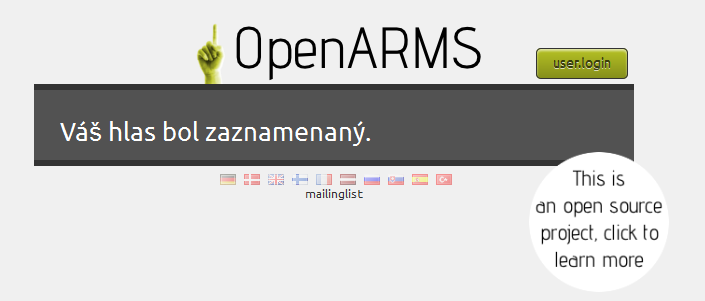
\includegraphics[scale=0.60]{pics/oA2.png}
\end{figure}
Technol�gie:
\begin{itemize}
 	\item    Java
  \item   Play! framework
 	\item    HTML
 	\item    JavaScript
\end{itemize}


\subsection{Pollin}

~~~~~ \url{http://hackday.linkedin.com/submission/entry/501d97cd268a5c874c0045f5} 

Closed-source projekt, ktor� bol vytvoren� na s��a�i LinkedIn Intern Hackday 2012. Stav projektu je moment�lne nezn�my, ale d� sa predpoklada�, �e tvorcovia sa pok�sia vytvori� komer�n� produkt, ktor� by bol konkuren�n� k n�mu projektu.

Pou�itie zah��a �kolsk� predn�ky, predn�ky na konferenci�ch a r�znych stretnutiach. Prezentuj�ci sa pomocou n�stroja m��e dozvedie� viac o publiku pomocou vytv�rania ankiet.

Implement�cia zahr�uje vytv�ranie prezent�ci�, ktor� m��u obsahova� ankety - publikum potom dostane webov� odkaz, ktor� poskytne rozhranie pre hlasovanie. Prezent�cie musia by� vytv�ran� pomocou n�stroja, tak�e predn�aj�ci je zna�ne obmedzen� pri vytv�ran� prezent�ci�.

Tento projekt bol v�sledkom 24 hodinovej s��a�e, no v praxi sa ned� pou�i�.

Technol�gie:
\begin{itemize}
	

  \item   YUI
  \item   JavaScript
  \item   Node.js
  \item  HTML5/CSS3
  \item   WebSockets
\end{itemize} 
%konceptualny datovy model
\section{Konceptu�lny d�tov� model}

\subsection{Popis z�kladn�ch ent�t}

\paragraph{Teacher} ~~~~~\\
 Entita Teacher reprezentuje pou��vate�a. Predpoklad� sa u�ite�, ktor� je v syst�me registrovan� a prihl�sen�.
Pri registr�cii sa vyplnia polo�ky name, fullname, password. Pre administr�tora je ur�en� polo�ka superuser.

\paragraph{Student} ~~~~~\\
Entita Student je jednou z k���ov�ch ent�t, preto�e uchov�va d�ta o pou��vate�och, ktor� nav�t�vili dan� anketu.
Klient sa identifikuje vo forme session id. �tudent m��e ma� priraden� svoje meno, ale nemus�. Z toho vypl�va, �e hlasovanie m��e by� do istej formy anonymn�.

\paragraph{Category}  ~~~~~\\
 Entita Category reprezentuje rozdelenie dotazn�kov do jednotliv�ch skup�n/kateg�ri� pre lep�iu spr�vu a preh�adnos�. 
Kateg�rie s� rozdelen� pod�a n�zvu a pr�stup k nim m� prihl�sen� pou��vate�.

\paragraph{Questionnaire} ~~~~~\\
Entita Questionnaire reprezentuje dan� dotazn�ky, ktor� sa nach�dzaj� v kateg�riach. Obsahuj� n�zov a public id, ktor� je potrebn� pri zobrazen� dan�ho dotazn�ka �tudentom.

\paragraph{Question} ~~~~~\\
Entita Question reprezentuje dan� ot�zky v syst�me. Questionnaire m��e obsahova� viacero ot�zok.
Medzi prvky, z ktor�ch pozost�va Question, patr� hlavne typ ot�zky. Tento typ m��e by� single, multi alebo text.
Pri single m��e by� ozna�en� jedna odpove�, pri multi m��e by� ozna�en�ch viacero odpoved� a pri text je po�adovan� odpove� v textovej forme.
�alej mo�nos� presented zna��, �i u� bola anketa publikovan� alebo nie. 

\paragraph{Comment} ~~~~~\\
Entita Comment reprezentuje koment�r k dan�mu Questionnaire. Cie� jej pou�itia je podpora sp�tnej v�zby. 
Pozost�va z mena (prez�vky) autora, nadpisu, tela, kde bude umiestnen� samotn� jadro koment�ra, a nakoniec �asu a d�tumu odoslania.

\paragraph{Option} ~~~~~\\
Entita Option obsahuje text konkr�tnej ot�zky. Vz�ahuje sa na entitu Question. Pre ka�d� mo�nos� je vytvoren� textov� reprezent�cia.

\paragraph{Answer} ~~~~~\\
Entita Answer sa vz�ahuje na entitu Question a entitu Student. �lohou je zaznamena�, �e bola prijat� konkr�tna odpove� na ot�zku. 

\paragraph{Rating} ~~~~~\\
Entita Rating sa vz�ahuje na entitu Questionnaire a entitu Student a poskytuje pou��vate�om (�tudentom) mo�nos� vyjardri� svoju spokojnos� s dan�m dotazn�kom t�m, �e mu daj� like alebo dislike. V�aka tejto entite sa n�sledne zobraz� �rove� spokojnosti s dotazn�kom.

\paragraph{StudentPresence} ~~~~~\\
T�to entita si uchov�va inform�cie o pr�tomnosti �tudentov (entita Student) na dotazn�koch (entita Questionnaire). Pou��va sa hlavne na zobrazenie po�tu �tudentov, ktor� si moment�lne prezeraj� dotazn�k.
~~~~~

\subsection{Logick� d�tov� model}
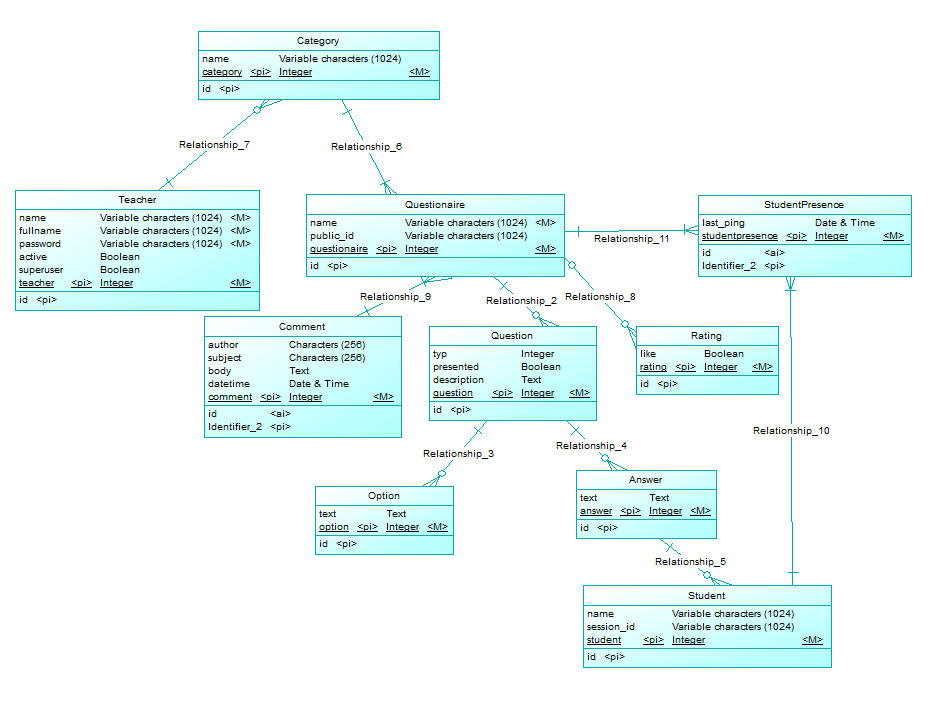
\includegraphics[scale=0.65]{pics/LogickyFinal.png}
\subsection{Fyzick� d�tov� model}
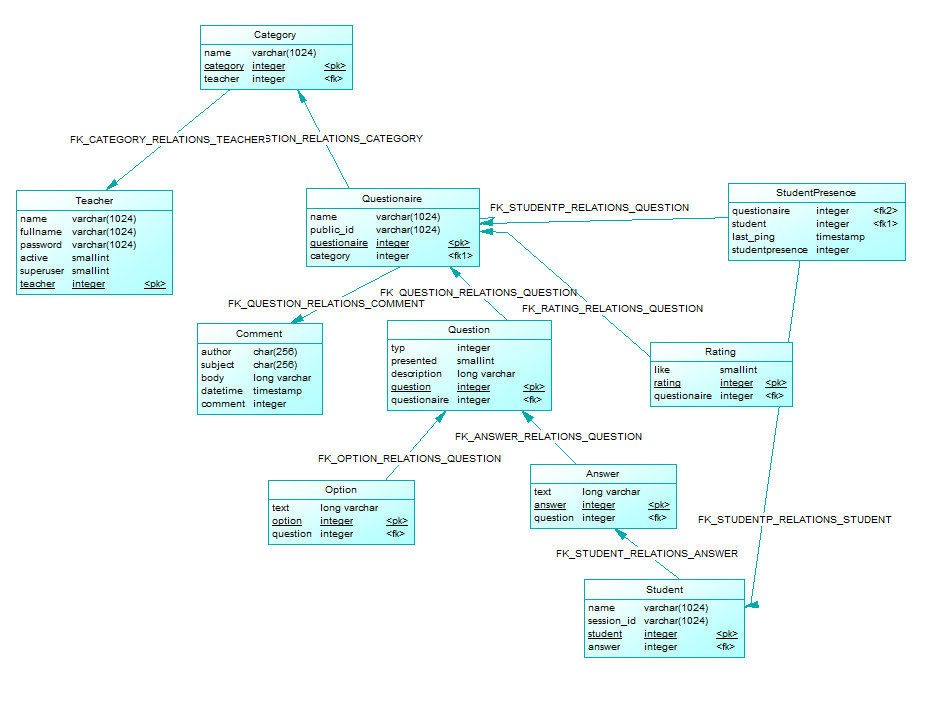
\includegraphics[scale=0.65]{pics/FyzickyFinal.png}

\subsection{Datab�zov� skript}
CREATE TABLE ��answer��
CREATE TABLE ��answer�� (��id�� INTEGER NOT NULL PRIMARY KEY, ��text�� TEXT, ��option\_id�� INTEGER NOT NULL REFERENCES ��option�� (��id��) , ��student\_id�� INTEGER NOT NULL REFERENCES ��student�� (��id��) ); 

CREATE TABLE ��category�� (��id�� INTEGER NOT NULL PRIMARY KEY, ��name�� VARCHAR(255) NOT NULL, ��teacher\_id�� INTEGER NOT NULL REFERENCES ��teacher�� (��id��) ); 

CREATE TABLE ��comment�� (��id�� INTEGER NOT NULL PRIMARY KEY, ��author�� VARCHAR(255) NOT NULL, ��subject�� VARCHAR(255) NOT NULL, ��body�� TEXT NOT NULL, ��questionnaire\_id�� INTEGER NOT NULL REFERENCES ��questionnaire�� (��id��) , ��datetime�� DATETIME NOT NULL); 

CREATE TABLE ��option�� (��id�� INTEGER NOT NULL PRIMARY KEY, ��text�� TEXT NOT NULL, ��question\_id�� INTEGER NOT NULL REFERENCES ��question�� (��id��) ); 

CREATE TABLE ��question�� (��id�� INTEGER NOT NULL PRIMARY KEY, ��description�� TEXT NOT NULL, ��typ�� INTEGER NOT NULL, ��presented�� SMALLINT NOT NULL, ��questionnaire\_id�� INTEGER NOT NULL REFERENCES ��questionnaire�� (��id��) ); 

CREATE TABLE ��questionnaire�� (��id�� INTEGER NOT NULL PRIMARY KEY, ��name�� VARCHAR(255) NOT NULL, ��public\_id�� VARCHAR(255) NOT NULL, ��category\_id�� INTEGER NOT NULL REFERENCES ��category�� (��id��) ); 

CREATE TABLE ��rating�� (��id�� INTEGER NOT NULL PRIMARY KEY, ��like�� SMALLINT NOT NULL, ��questionnaire\_id�� INTEGER NOT NULL REFERENCES ��questionnaire�� (��id��) ); 

CREATE TABLE ��student�� (��id�� INTEGER NOT NULL PRIMARY KEY, ��name�� VARCHAR(255) NOT NULL, ��session\_id�� VARCHAR(255) NOT NULL); 

CREATE TABLE ��teacher�� (��id�� INTEGER NOT NULL PRIMARY KEY, ��username�� VARCHAR(255) NOT NULL, ��fullname�� VARCHAR(255) NOT NULL, ��email�� VARCHAR(255) NOT NULL, ��password�� VARCHAR(255) NOT NULL, ��active�� SMALLINT NOT NULL, ��superuser�� SMALLINT NOT NULL);

CREATE INDEX ��answer\_option\_id�� ON ��answer�� (��option\_id��);

CREATE INDEX ��answer\_student\_id�� ON ��answer�� (��student\_id��);

CREATE INDEX ��category\_teacher\_id�� ON ��category�� (��teacher\_id��);

CREATE INDEX ��comment\_questionnaire\_id�� ON ��comment�� (��questionnaire\_id��);

CREATE INDEX ��option\_question\_id�� ON ��option�� (��question\_id��);

CREATE INDEX ��question\_questionnaire\_id�� ON ��question�� (��questionnaire\_id��);

CREATE INDEX ��questionnaire\_category\_id�� ON ��questionnaire�� (��category\_id��);

CREATE INDEX ��questionnaire\_name\_category\_id�� ON ��questionnaire�� (��name��, ��category\_id��);

CREATE UNIQUE INDEX ��questionnaire\_public\_id�� ON ��questionnaire�� (��public\_id��);

CREATE INDEX ��rating\_questionnaire\_id�� ON ��rating�� (��questionnaire\_id��);

%detailny navrh
\section{N�vrh aplik�cie}

~~~~~


\subsection{Pou�it� technol�gie}
~~~~~ Technol�gie, ktor� boli pou�it� pri vytv�ran� tejto webovej aplik�cie.


\subsubsection{Klientsk� �as�}

 \begin{itemize}
   \item      programovac� jazyk CoffeeScript skompilovan� do JavaScriptu
   \item      MVC framework Spine (\url{http://spinejs.com/})
   \item      D3 kni�nica
   \item      Kni�nica pre manipul�ciu DOM, jQuery (\url{http://jquery.com})
   \item      CSS3
 \end{itemize}


\subsubsection{Serverov� �as�}

 \begin{itemize}

   \item      programovac� jazyk Python
   \item      microframework Flask (\url{http://flask.pocoo.org/})
   \item      ORM framework peewee (\url{http://peewee.readthedocs.org})
   \item      datab�za SQLite
   \item      moduly
   \subitem �tudent
   \subitem u�ite�
 \end{itemize}
            
    
 
\subsection{Detailn� n�vrh aplik�cie}
    
    
    
\subsubsection{Registr�cia}    
 Registr�cia pou��vate�a prebieha pomocou formul�ra. Pou��vate� vypln� formul�r v tvare prez�vka, pou��vate�sk� meno, heslo a email.
 N�sledne potvrd� stla�en�m tla�idla Odosla�.
 
\begin{figure}[h!]
\centering
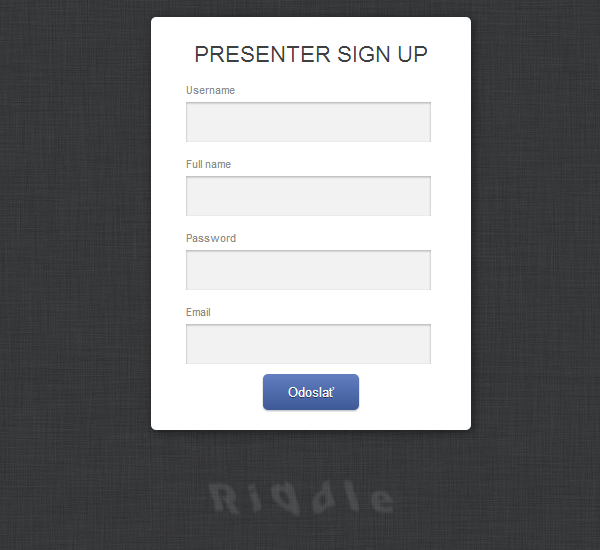
\includegraphics[scale=0.65]{pics/registraciaCROP.png}
\end{figure}

\newpage
\subsubsection{Prihl�senie} 
 Prihl�senie pou��vate�a prebieha pomocou formul�ru, kde pou��vate� zad� svoju prez�vku a heslo.
 N�sledne potvrd� stla�en�m tla�idla Odosla�. \\
 Po �spe�nom prihl�sen� ho aplik�cia presunie na str�nku obsahuj�cu kateg�rie a pod nich spadaj�ce dotazn�ky.
 
\begin{figure}[h!]
\centering
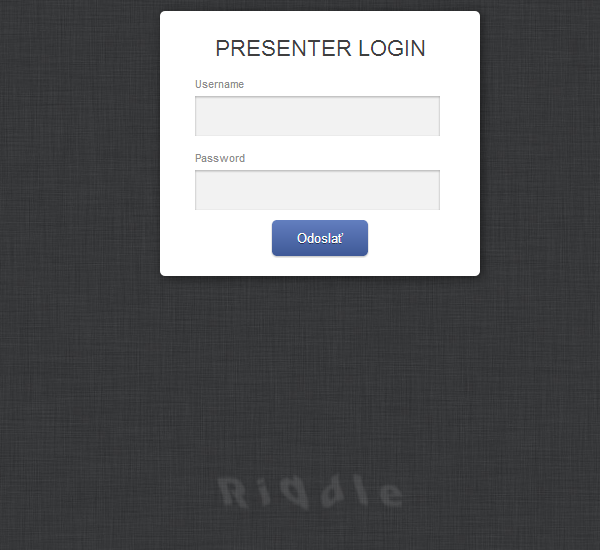
\includegraphics[scale=0.65]{pics/loginCROP.png}
\end{figure}   

\newpage
\subsubsection{Spr�va dotazn�kov}   
Na tejto str�nke pou��vate� preh�adne vid� svoje vytvoren� dotazn�ky rozdelen� do kateg�ri�. \\
V pravom hornom rohu aplik�cie sa nach�dza meno pou��vate�a a pod n�m mo�nos� odhl�senia sa z aplik�cie.\\
Po kliknut� na dan� dotazn�k sa pou��vate�ovi otvor� okno, kde uvid� zoznam ot�zok, ktor� dotazn�k obsahuje.\\
Po kliknut� na tla�idlo Add category sa pou��vate�ovi zobraz� okno, kde m��e prida� nov� kateg�riu.\\
Po kliknut� na tla�idlo Edit m� mo�nos� upravi� dotazn�k.\\
Pre r�chle vytvorenie nov�ho dotazn�ka je k dispoz�cii v�dy na konci kateg�rie tla�idlo Add lecture.

\begin{figure}[h!]
\centering
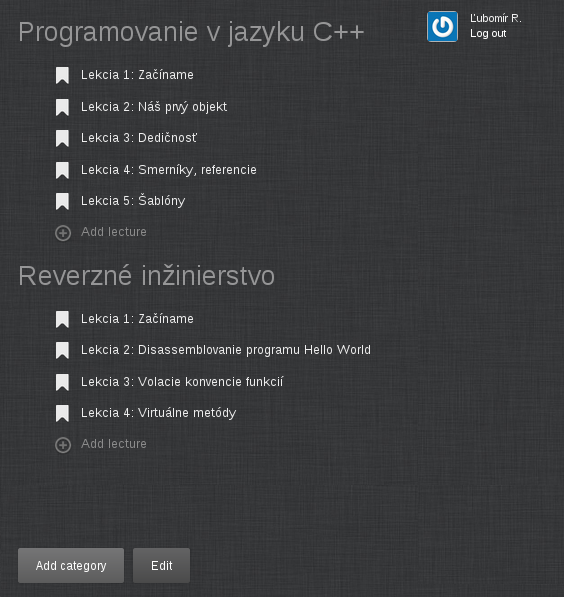
\includegraphics[scale=0.90]{pics/dashboardCROP.png}
\end{figure}

\newpage
\subsubsection{Pridanie kateg�rie}   
Na tejto str�nke m� pou��vate� mo�nos� prida� nov� kateg�riu, a to zadan�m n�zvu novej kateg�rie a n�sledn�m kliknut�m na tla�idlo Odosla�.
Potom bude presmerovan� nasp� na str�nku so spr�vou dotazn�kov. 
\begin{figure}[h!]
\centering
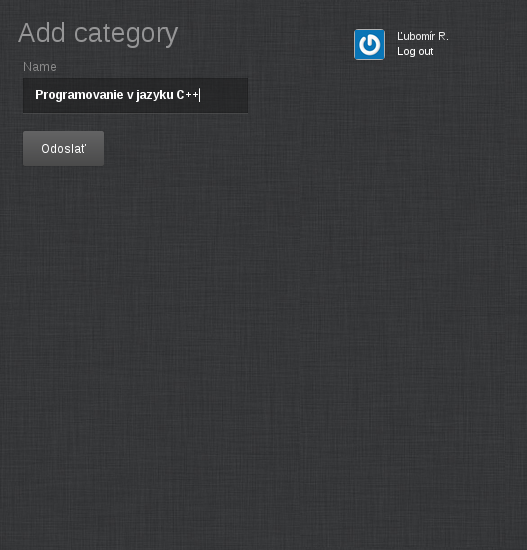
\includegraphics[scale=0.75]{pics/add-categoryCROP.png}
\end{figure}

\newpage
\subsubsection{Zobrazenie ot�zok}     
Na tejto str�nke pou��vate� vid� zoznam ot�zok vytvoren�ch v tomto dotazn�ku.\\
Pri ka�dej ot�zke je mo�nost editova�, zmaza� alebo prezentova� dan� ot�zku. \\
Pri ozna�en� ot�zky prezentova� stla�en�m tla�idla Present sa stane ot�zka vidite�nou pre �tudentov.\\
V spodnej �asti sa nach�dzaj� tla�idl� ur�en� na pridanie ot�zky a prezentovanie.
\begin{figure}[h!]
\centering
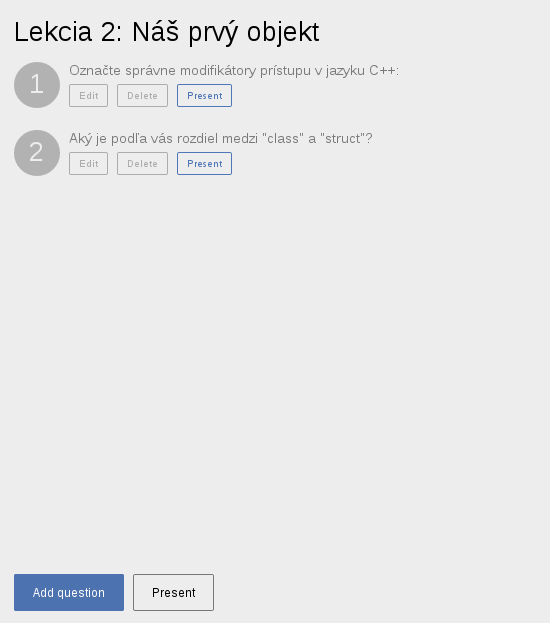
\includegraphics[scale=0.75]{pics/view-questionsCROP.png}
\end{figure}

\newpage
\subsubsection{�prava dotazn�ka}    
Na tejto str�nke m� pou��vate� mo�nos� upravi� dotazn�k. \\
V�avej hornej �asti je pole ozna�en� ako Title, kde je mo�n� zmeni� n�zov ot�zky.\\
Pod n�m je combo box s mo�nos�ou zmeny typu ot�zky z multiple choice na sigle choice alebo textov�.\\
V pravej �asti sa nach�dzaj� polia s aktu�lnymi mo�nos�ami.\\
Hore sa nach�dza tla�idlo, ktor� prid� �al�iu mo�nos�.\\
�alej je mo�n� premenova� aktu�lne mo�nosti.\\
\begin{figure}[h!]
\centering
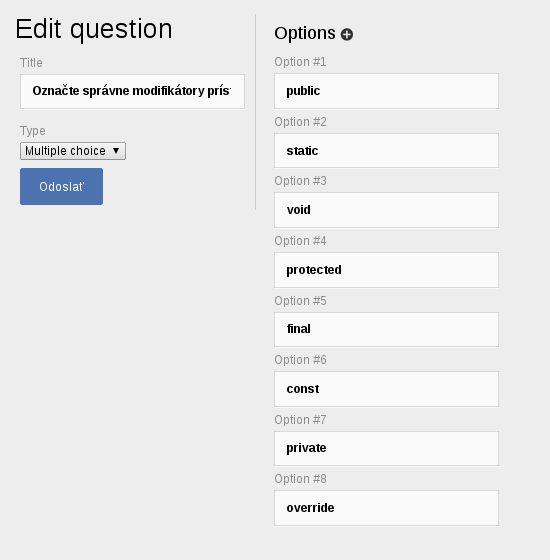
\includegraphics[scale=0.75]{pics/add-questionCROP.png}
\end{figure}

\newpage
\subsubsection{Publikovanie dotazn�ka}     
Pri publikovan� dotazn�ka sa zobraz� QR k�d a link na str�nku, kde m��u �tudenti hlasova�.
\begin{figure}[h!]
\centering
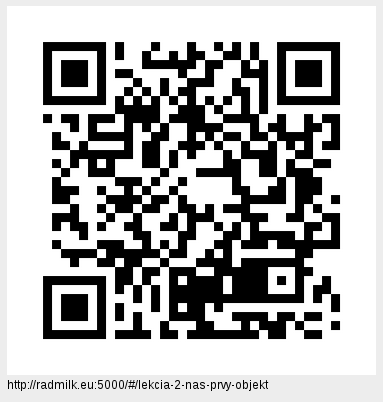
\includegraphics[scale=0.75]{pics/qrANDlinkCROP.png}
\end{figure}

\newpage
\subsubsection{Mo�nos� odoslania}     
T�to str�nka d�va �tudentovi vybra� mo�nos� zada� svoju prez�vku, alebo osta� anonymn�.
\begin{figure}[h!]
\centering
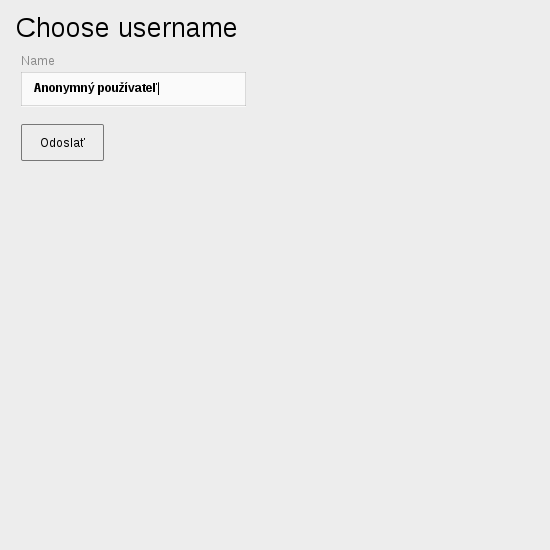
\includegraphics[scale=0.75]{pics/choose-usernameCROP.png}
\end{figure}

\newpage
\subsubsection{Prezentovan� ot�zka}     
T�to str�nka reprezentuje �o uvid� �tudent pri nav�t�ven� zverejnen�ho dotazn�ka. \\
V hornej �asti str�nky je umiestnenie danej ot�zky (kateg�ria-dotazn�k).\\
�alej je n�zov ot�zky a prezentovan� mo�nosti.\\
V dolnej �asti je mo�nos� prida� koment�r.\\
Nakoniec sa to v�etko odo�le stla�en�m tla�idla Odosla�.\\
\begin{figure}[h!]
\centering
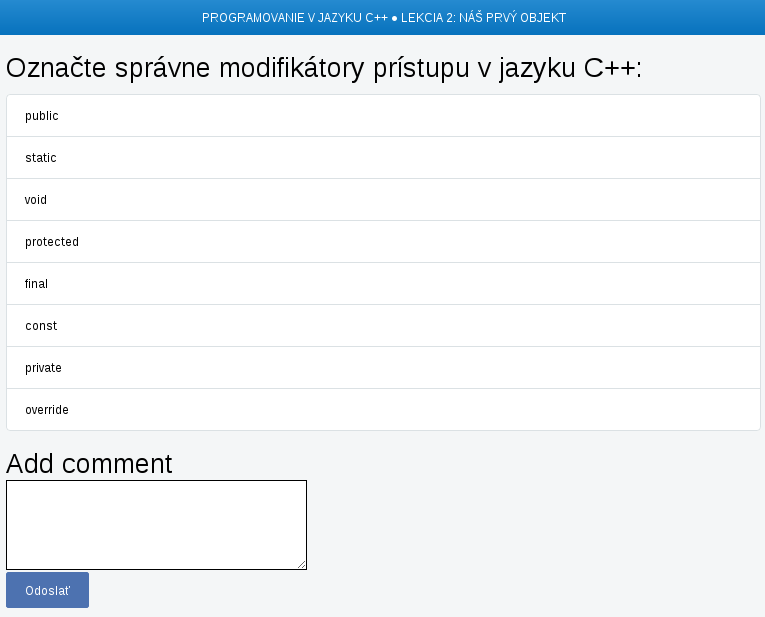
\includegraphics[scale=0.60]{pics/student-questionCROP.png}
\end{figure}

\newpage
\subsubsection{Vyhodnotenie ot�zky}   
Na tejto str�nke sa nach�dza vyhodnotenie ot�zky vo forme grafu reprezentuj�ceho po�et hlasov pre dan� mo�nos�.
\begin{figure}[h!]
\centering
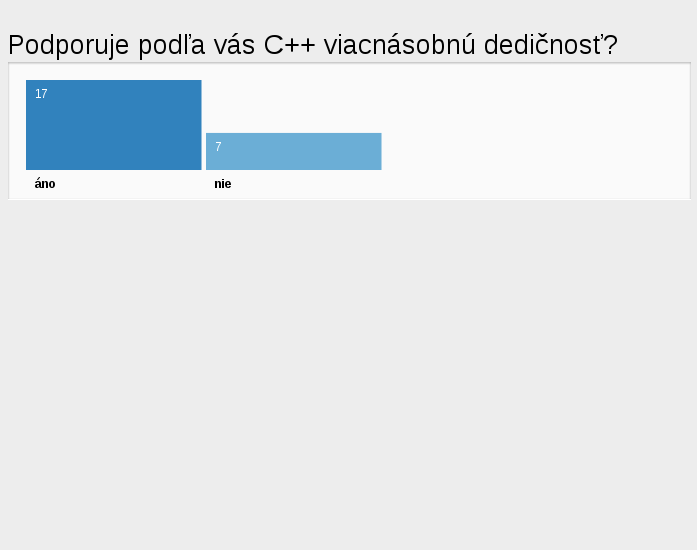
\includegraphics[scale=0.60]{pics/questionnaire-resultsCROP.png}
\end{figure}
%use case
\section{Use cases.}
~~~~~ Pr�pady pou�itia (Use cases).

 \subsection{Teacher}

 	\subsubsection{Registr�cia.}
\begin{enumerate}
	\item Aplik�cia vy�iada registra�n� �daje.
	\item U�ite� (�alej len pou��vate�) zad� registra�n� �daje (meno, priezvisko, heslo, e-mail).
	\item Aplik�cia over� registra�n� �daje.
	\item Aplik�cia vytvor� nov�ho pou��vate�a v syst�me.
\end{enumerate}

 	\subsubsection{Prihl�senie.}
\begin{enumerate}
	\item Aplik�cia vy�iada prihlasovacie �daje.
	\item Pou��vate� zad� prihlasovacie �daje (meno, heslo).
	\item Aplik�cia over� prihlasovacie �daje.
	\item Aplik�cia prihl�si pou��vate�a.
	\item Aplik�cia spr�stupn� funkcie pre spr�vu dotazn�kov.
\end{enumerate}

 	\subsubsection{Spr�va dotazn�kov.}
 	\begin{enumerate}
	\item Aplik�cia zobraz� u� vytvoren� dotazn�ky rozdelen� do kateg�rii.
	\item Pou��vate� m��e vytvori� nov� dotazn�k, alebo zverejni� u� vytvoren�.
	\item Pri zverejnen� dotazn�ka aplik�cia nastav� premenn� published pre dan� dotazn�k na true a vygeneruje link a QR k�d.  
	\item Link a QR k�d zobraz� pou��vate�ovi.
	\item N�sledne m��u �tudenti pristupova� na str�nku.
\end{enumerate}
 
  \subsubsection{Vytvorenie/Nastavenie dotazn�ka}
 	\begin{enumerate}
	\item Pou��vate� si zvol� mo�nos� vytvori� nov� dotazn�k v u� existuj�cej kateg�rii, pr�padne vytvor� nov� kateg�riu a v nej nov� dotazn�k.
	\item V novom dotazn�ku si zvol� typy ot�zok a �ubovoln� po�et ot�zok.
	\item Aplik�cia ulo�� vytvoren� dotazn�k do datab�zy.
	\end{enumerate}
 	
  	\subsubsection{Zobrazenie v�sledkov.}
 	\begin{enumerate}
	\item Pou��vate� si zvol� konkr�tnu ot�zku v dotazn�ku.
	\item Aplik�cia mu v re�lnom �ase zobrazuje vyhodnotenie ot�zky v textovej aj grafickej podobe.
\end{enumerate}

 \subsection{Student}
 
 	\subsubsection{Hlasovanie.}
 	\begin{enumerate}
	\item �tudent prist�pi na str�nku zverejnen�ho dotazn�ka.
	\item Vyplni� m��e anonymne alebo m��e nap�sa� svoje meno.
	\item Po vyplnen� dotazn�ka odo�le �daje.
	\item Aplik�cia spracuje prijat� �daje a okam�ite aktualizuje grafick� alebo textov� zobrazenie.

\end{enumerate}
  ~~~~~ 
  \subsubsection{Sp�tn� v�zba.}
   	\begin{enumerate}
  \item �tudent prist�pi na str�nku zverejnen�ho dotazn�ka.
	\item �tudent m��e nap�sa� koment�r k dotazn�ku alebo da� svoj like alebo dislike.
	\item Aplik�cia spracuje �daje a spr�stupn� prihl�sen�mu pou��vate�ovi mo�nosti prezrie� si koment�re.
	\item Aplik�cia na str�nke s vyhodnoten�m �dajov hlasovania zobraz� graf v podobe po�tu like-ov a dislike-ov.
	\end{enumerate}
	

%pouzita literatura
\section{Pou�it� literat�ra}

\url{http://flask.pocoo.org/docs/} \\
\url{http://flask-peewee.readthedocs.org/en/latest/} \\
\url{http://spinejs.com/docs/index}  \\



\bibliographystyle{abbrv}
\bibliography{simple}

\end{document}
This is never printed
